\documentclass[conference]{IEEEtran}
\usepackage{graphicx}
\usepackage{booktabs}
\usepackage{amsmath}
\usepackage{url}
\graphicspath{{./}}

\begin{document}

\title{RL-Adaptive Deception for Protecting Post-Quantum IoT Gateways from Reconnaissance and Downgrade Attacks}

\author{\IEEEauthorblockN{Zyeem Bin Zia}
\IEEEauthorblockA{Independent Researcher, Bangladesh\\
zyeemzia@gmail.com}}

\maketitle

\begin{abstract}
The migration of IoT gateways to post-quantum key establishment exposes a new
pre-authentication attack surface: adversaries can fingerprint the ML-KEM service,
request fallback to classical key exchange, and flood the comparatively expensive
handshake. We present a reinforcement-learning (RL) deception defender that routes
each incoming request either to a real ML-KEM-768 service running on an ESP32
microcontroller or to a decoy whose compute timing is calibrated to measurements
from that device. We measure ML-KEM-768 on the ESP32 (240\,MHz, portable C):
8.17\,ms key generation, 9.39\,ms encapsulation and 11.15\,ms decapsulation with a
15.1\,KB peak stack ($n=100$), and 100 end-to-end WiFi handshakes with key
confirmation. These measurements parameterise a Gymnasium environment with five
attacker profiles and mixed legitimate traffic. Across five seeds and 200 held-out
episodes each, a QR-DQN defender deflects 98.6\% of reconnaissance requests
(static rule: 76.0\%), captures 42.7\% of downgrade attempts (32.2\%), and
sustains attacker engagement 3.8$\times$ longer, with a 0.6\% legitimate
false-positive rate. QR-DQN outperforms the static rule in 15/15 runs of a
sensitivity analysis that perturbs reward weights, decoy-detection probabilities,
and traffic mix by $\pm$50\%. Code, raw measurements and trained models are
available at \url{https://github.com/zyeemzia/pqc-deception-honeypot}.
\end{abstract}

\begin{IEEEkeywords}
post-quantum cryptography, ML-KEM, cyber deception, reinforcement learning, IoT security, ESP32
\end{IEEEkeywords}

\section{Introduction}
NIST standardised ML-KEM as FIPS~203 in 2024~\cite{fips203}, and IoT
deployments are beginning to adopt post-quantum key establishment. Much work
evaluates the cost of running ML-KEM on constrained hardware; less attention has
been paid to the operational attack surface of the handshake itself. Before
authentication, an attacker can (i) fingerprint the service to confirm the device
and implementation, (ii) attempt to downgrade to a classical key exchange during
the migration period, and (iii) flood the handshake endpoint.

Cyber deception is an established response to reconnaissance, and RL has been
used to adapt honeypot behaviour to attackers~\cite{honeyiot}. We apply
RL-adaptive deception to the post-quantum handshake of an IoT gateway and ground
it in measurements from real constrained hardware rather than simulated costs.

\textbf{Contributions.}
\begin{itemize}
\item On-device measurements of ML-KEM-768 (PQClean~\cite{pqclean}) on an ESP32:
latency, memory, and 100 networked handshakes with key confirmation over WiFi.
\item A decoy gateway that performs genuine ML-KEM but pads its compute time to the
measured ESP32 distribution.
\item A Gymnasium environment for gateway deception, with five attacker profiles
mapped to MITRE ATT\&CK~\cite{attack} and latency costs sampled from real data.
\item An evaluation of QR-DQN~\cite{qrdqn} and DQN~\cite{dqn} against three
baselines over five seeds, with paired significance tests, a sensitivity analysis,
and an attacker-behaviour classifier.
\end{itemize}

\section{Related Work}
\textbf{ML-KEM on constrained devices.} The pqm4 framework~\cite{pqm4} is the
de facto platform for benchmarking post-quantum schemes on Arm Cortex-M4
microcontrollers. On the ESP32, Azevedo \emph{et al.}~\cite{azevedo} selectively
parallelise ML-KEM-512 across the chip's two cores, reducing the total
KeyGen+Encaps+Decaps time from 27.7\,ms to 19.6\,ms (about 1.41$\times$). Nagy
\emph{et al.}~\cite{nagy} report that their attempts to run ML-KEM on ESP32 and
other microcontroller boards were unsuccessful due to memory constraints, and
benchmark on a Raspberry Pi 4B instead. In contrast, we run the portable PQClean
ML-KEM-768 implementation on an ESP32 in a dedicated task with an enlarged stack
and report its measured peak stack (15.1\,KB). Our measurements are a baseline
cost for the defender, not an optimisation contribution, and we do not claim to be
the first to run ML-KEM on this platform.

\textbf{RL for honeypots and deception.} HoneyIoT~\cite{honeyiot} formulates an
adaptive IoT honeypot as an MDP learned with RL. Our environment adopts a similar
interaction structure but addresses a different asset (a post-quantum handshake)
and adds legitimate traffic, so that the defender faces a false-positive trade-off.

\textbf{Post-quantum deception frameworks.} QuantumGuard~\cite{quantumguard}
combines RL-driven deception with CRYSTALS-Kyber/Dilithium to secure an
intelligence-sharing channel between defender organisations, with cryptographic
costs measured on server-class hardware. Our work instead protects the
key-establishment endpoint of a single constrained device and measures its
cryptographic cost on that device.

\section{Threat Model}
The protected asset is an ESP32 gateway that establishes session keys with
ML-KEM-768 and refuses classical fallback. The attacker can connect to the
gateway, grab its banner, perform protocol-conformant handshakes as timing probes,
request a classical ECDH fallback, and flood handshake requests. The attacker
cannot break ML-KEM, compromise firmware, or observe the defender's state.
Physical and side-channel attacks are out of scope. The defender runs at the
gateway, observes each request with limited source history, and may route it to
the real service, a low- or high-fidelity decoy, a throttled real service, or
block the source.

\section{System and Hardware Measurements}
\subsection{Real service}
The gateway firmware (Arduino-ESP32, PlatformIO) links the PQClean
\texttt{ml-kem-768/clean} sources and uses the ESP32 hardware RNG. For a
handshake, the gateway generates a key pair, sends the 1184-byte public key,
receives the 1088-byte ciphertext, decapsulates, and returns SHA3-256 of the
shared secret as key confirmation. A downgrade request is refused and logged.
Fig.~\ref{fig:board} shows the device used for all measurements.

\begin{figure}[t]
\centering
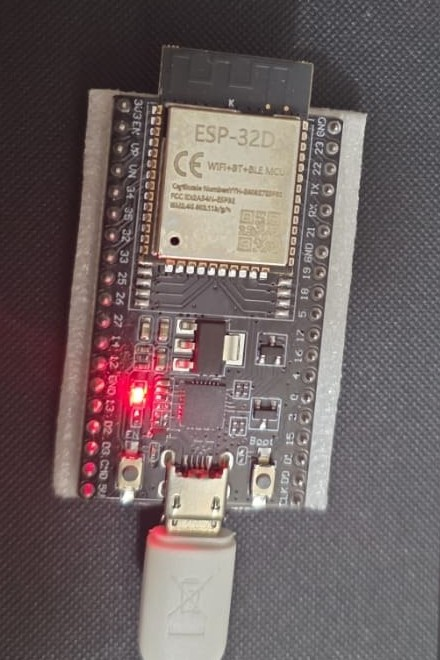
\includegraphics[width=0.5\columnwidth]{esp32_testbed.jpg}
\caption{The ESP32 DevKit (ESP-32D module, CP2102 USB-UART) that ran every
ML-KEM-768 measurement and served the real gateway.}
\label{fig:board}
\end{figure}

\subsection{On-device cost}
Table~\ref{tab:hw} reports 100 consecutive KeyGen/Encaps/Decaps runs at
240\,MHz with WiFi disabled. All runs produced matching shared secrets. Peak
stack usage was 15{,}096 bytes and free heap never fell below 291{,}448 bytes.
The peak stack alone exceeds the $\sim$10\,KiB RAM of an RFC~7228 Class-1
device~\cite{rfc7228}, which motivates placing the adaptive defender at the
gateway rather than on end nodes.

\begin{table}[t]
\centering
\caption{ML-KEM-768 on ESP32 (240\,MHz, PQClean clean C, $n=100$).}
\label{tab:hw}
\begin{tabular}{lcccc}
\toprule
Operation & Mean (ms) & Std & Min & Max \\
\midrule
KeyGen & 8.171 & 0.099 & 8.145 & 9.104 \\
Encaps & 9.390 & 0.033 & 9.372 & 9.527 \\
Decaps & 11.150 & 0.030 & 11.133 & 11.247 \\
\bottomrule
\end{tabular}
\end{table}

\subsection{Networked handshakes}
With the ESP32 as server on a shared 2.4\,GHz institutional WLAN and a laptop
client performing encapsulation with kyber-py, all 100 handshakes passed key
confirmation. On-device KeyGen and Decaps were $8.64\pm0.03$\,ms and
$11.60\pm0.03$\,ms. Total handshake time had a median of 320.8\,ms (mean
1249.8\,ms, 90th percentile 3332.7\,ms), and 25/100 handshakes exceeded 1\,s:
latency was dominated by the wireless link rather than by ML-KEM computation.

\subsection{Decoy}
The decoy speaks the same protocol and performs genuine ML-KEM, so key and
ciphertext sizes and formats match. Its reported and actual compute times are
padded to samples drawn from the measured ESP32 distributions. In a local test
($n=30$) the decoy's reported KeyGen and Decaps times were $8.64\pm0.03$\,ms and
$11.60\pm0.02$\,ms, matching the device.

\section{RL Environment and Agents}
\textbf{Episodes.} Each 60-step episode contains one attacker drawn from five
profiles (scanner, downgrader, flooder, multi-stage APT, stealthy prober) and
legitimate clients that issue 35\% of requests. Attackers progress through
kill-chain stages (Reconnaissance TA0043, Defense Evasion TA0005, Impact TA0040).

\textbf{Observation} (12 features): request type (one-hot), the source's prior
request counts per type, whether the source has seen a decoy, request rate,
episode progress, and whether the attacker suspects deception.

\textbf{Actions:} route to real service, low-fidelity decoy, high-fidelity decoy,
throttle, or block. An attacker routed to a decoy detects it with probability
0.25 (low fidelity) or 0.05 (high fidelity) per interaction and then leaves.

\textbf{Reward.} Positive terms for attacker engagement, recon deflection and
downgrade capture; negative terms for recon leakage, downgrade requests reaching
the device, floods reaching the device, misrouting or blocking legitimate
clients, and legitimate-client latency. Latency is sampled from the 100 measured
WiFi handshakes.

\textbf{Agents.} QR-DQN (50 quantiles) and DQN from SB3-Contrib and
Stable-Baselines3~\cite{sb3} with a $128\times128$ MLP, $2\times10^5$ steps,
learning rate $5\times10^{-4}$, $\gamma=0.97$, batch 128, replay buffer $10^5$,
$\epsilon$ annealed to 0.02 over 30\% of training. Environments follow the
Gymnasium API~\cite{gymnasium}.

\textbf{Baselines.} No deception (always real), random routing, and a static rule
that sends handshakes to the real service and all other requests to the
low-fidelity decoy.

\section{Evaluation}
\subsection{Protocol}
Each agent is trained with seeds 42, 123, 456, 789 and 1024 and evaluated on 200
episodes per seed whose seeds are disjoint from training. The unit of analysis is
the seed ($n=5$): per-seed means are compared with paired $t$-tests when
differences pass Shapiro--Wilk, otherwise Wilcoxon signed-rank.

\subsection{Main results}
Table~\ref{tab:main} and Fig.~\ref{fig:main} summarise the results. QR-DQN
outperforms the static rule in return ($p<0.0001$) and recon deflection
(98.6\% vs 76.0\%, $p=0.0001$), captures more downgrade attempts (42.7\% vs
32.2\%), and keeps attackers engaged for 15.6 vs 4.1 steps, largely by using the
high-fidelity decoy: the static rule's low-fidelity decoy is detected in almost
every episode (0.999 detections per episode). The cost is a 0.6\%
legitimate false-positive rate versus 0\% for the static rule ($p=0.0115$).
QR-DQN and DQN reach similar returns ($p=0.14$); QR-DQN has fewer false positives
(0.6\% vs 3.0\%, $p=0.0085$).

\begin{table*}[t]
\centering
\caption{Held-out evaluation (mean $\pm$ std over 5 seeds, 200 episodes each).}
\label{tab:main}
\begin{tabular}{lccccc}
\toprule
Policy & Return & Recon deflected & Downgrade captured & Legit FP rate & Engagement (steps) \\
\midrule
No deception & $-139.8\pm2.2$ & 0.000 & 0.000 & 0.000 & 0.0 \\
Random & $-178.6\pm1.3$ & $0.364\pm0.035$ & $0.030\pm0.006$ & $0.402\pm0.005$ & $1.6\pm0.1$ \\
Static rule & $-33.1\pm1.9$ & $0.760\pm0.024$ & $0.322\pm0.027$ & 0.000 & $4.1\pm0.3$ \\
DQN & $12.5\pm4.2$ & $0.995\pm0.006$ & $0.400\pm0.051$ & $0.030\pm0.012$ & $16.4\pm0.9$ \\
QR-DQN & $15.4\pm4.4$ & $0.986\pm0.008$ & $0.427\pm0.038$ & $0.006\pm0.003$ & $15.6\pm1.2$ \\
\bottomrule
\end{tabular}
\end{table*}

\begin{figure*}[t]
\centering
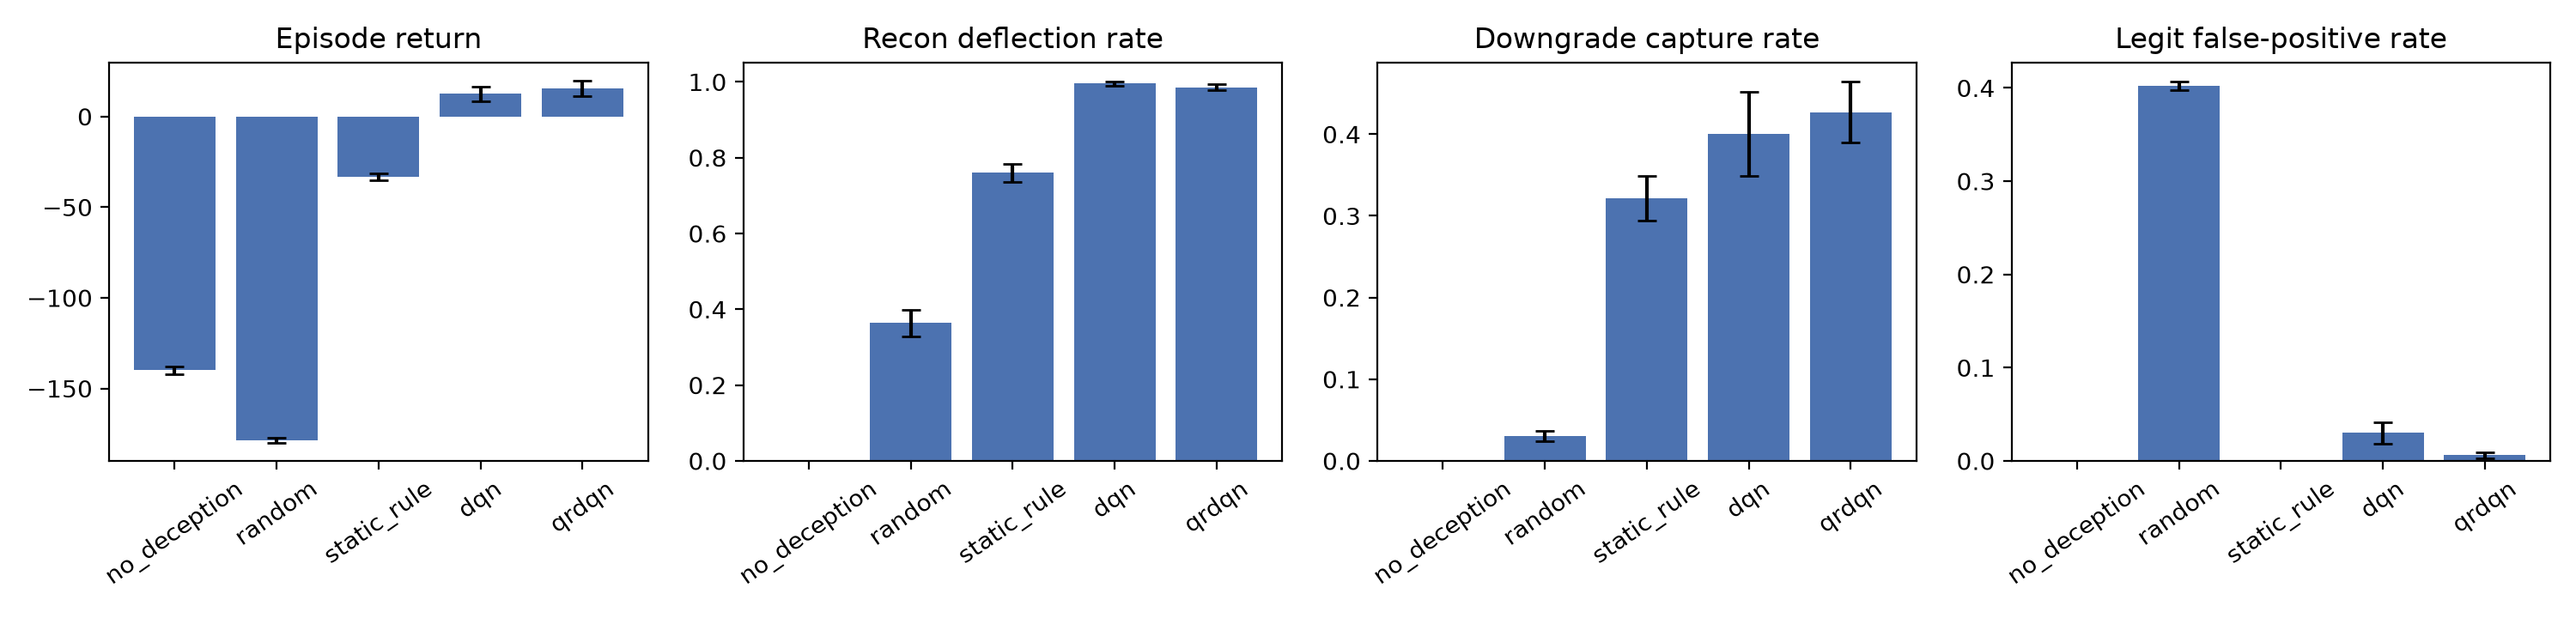
\includegraphics[width=\textwidth]{policy_comparison.png}
\caption{Policy comparison on held-out episodes (error bars: std over 5 seeds).}
\label{fig:main}
\end{figure*}

\subsection{Sensitivity analysis}
Because reward weights and detection probabilities are design choices, we retrain
QR-DQN (3 seeds each) under five perturbed settings: positive rewards $\times0.5$,
penalties $\times1.5$, detection probability $\times1.5$ and $\times0.5$, and
legitimate traffic raised to 50\%. QR-DQN's return exceeded the static rule's in
all 15 runs (Table~\ref{tab:sens}). Recon deflection stayed between 91.5\% and
98.3\% and false positives at or below 0.6\%. Variance was highest when decoys
were harder to detect (return std 22.8).

\begin{table}[t]
\centering
\caption{Sensitivity: QR-DQN vs static rule (mean over 3 seeds).}
\label{tab:sens}
\begin{tabular}{lccc}
\toprule
Condition & QR-DQN & Static & QR-DQN deflect. \\
\midrule
Positive rewards $\times0.5$ & $-38.0$ & $-54.2$ & 0.983 \\
Penalties $\times1.5$ & $-27.6$ & $-71.1$ & 0.950 \\
Detection $\times1.5$ & $-0.4$ & $-39.5$ & 0.965 \\
Detection $\times0.5$ & $22.2$ & $-18.1$ & 0.983 \\
Legit traffic 50\% & $3.5$ & $-33.1$ & 0.915 \\
\bottomrule
\end{tabular}
\end{table}

\subsection{Attacker-behaviour classification}
Sessions observed at the decoy are classified into the five attacker profiles
and legitimate clients using 14 features (request counts and fractions, rate
statistics, request-sequence entropy, transitions, first request). With 5-fold
stratified cross-validation repeated over five seeds, Random Forest reached
macro-F1 $0.921\pm0.007$ and XGBoost $0.912\pm0.008$. Scanners were hardest to
separate (F1 0.877) because they resemble the first stage of the APT profile.
Classes are mapped to ATT\&CK: T1595 Active Scanning, T1562.010 Downgrade Attack,
and T1499 Endpoint Denial of Service. These scores are on simulated sessions and
validate the pipeline, not real-world detection.

\section{Limitations}
(i) Attackers follow scripted profiles and are not deception-aware beyond a
per-interaction detection probability; adaptive adversaries are future work.
(ii) Reward weights are design choices; the sensitivity analysis covers
$\pm$50\% perturbations with three seeds, not an exhaustive search.
(iii) The decoy matches the device's compute-time fingerprint, but not the
network-path fingerprint unless it is hosted behind the same link.
(iv) Results use one device, one parameter set (ML-KEM-768), a portable C
implementation without assembly optimisation, and one shared WLAN.
(v) The on-device benchmark ran with the radio off, so the hardware RNG was not
fully radio-seeded; networked runs had WiFi enabled.

\section{Conclusion}
We showed that RL-adaptive deception can protect a post-quantum IoT gateway's
handshake with costs grounded in real ESP32 measurements. A QR-DQN defender
deflected 98.6\% of reconnaissance, captured 42.7\% of downgrade attempts, and
kept attackers engaged 3.8$\times$ longer than a static rule, at a 0.6\%
false-positive cost, and this advantage persisted across perturbed reward and
detection settings. Future work includes deception-aware adversaries, decoys
hosted on the gateway to match network-path fingerprints, and optimised ML-KEM
implementations.

\begin{thebibliography}{99}
\bibitem{fips203} National Institute of Standards and Technology,
``Module-Lattice-Based Key-Encapsulation Mechanism Standard,'' FIPS 203, Aug. 2024.
\bibitem{rfc7228} C. Bormann, M. Ersue, and A. Keranen, ``Terminology for
Constrained-Node Networks,'' RFC 7228, IETF, May 2014.
\bibitem{pqclean} M. J. Kannwischer, P. Schwabe, D. Stebila, and T. Wiggers,
``Improving software quality in cryptography standardization projects,'' in
Proc. IEEE EuroS\&P Workshops (SSR), 2022. IACR ePrint 2022/337.
\bibitem{pqm4} M. J. Kannwischer \emph{et al.}, ``pqm4: Post-quantum crypto
library for the ARM Cortex-M4,'' \url{https://github.com/mupq/pqm4}.
\bibitem{azevedo} B. L. Azevedo, V. Lagrota, and M. V. Ribeiro, ``Multicore
implementation of ML-KEM on embedded devices,'' in Proc. 25th Simp\'osio
Brasileiro de Ciberseguran\c{c}a (SBSeg), 2025, pp. 659--675,
doi: 10.5753/sbseg.2025.9783.
\bibitem{nagy} N. Nagy, S. Alnemer, L. M. Alshuhail, H. Alobiad, T. Almulla,
F. A. Alrumaihi, N. Ghadra, and M. Nagy, ``Module-lattice-based key-encapsulation
mechanism performance measurements,'' \emph{Sci}, vol. 7, no. 3, art. 91, 2025,
doi: 10.3390/sci7030091.
\bibitem{qrdqn} W. Dabney, M. Rowland, M. G. Bellemare, and R. Munos,
``Distributional reinforcement learning with quantile regression,'' in Proc.
AAAI, 2018.
\bibitem{dqn} V. Mnih \emph{et al.}, ``Human-level control through deep
reinforcement learning,'' \emph{Nature}, vol. 518, pp. 529--533, 2015.
\bibitem{sb3} A. Raffin, A. Hill, A. Gleave, A. Kanervisto, M. Ernestus, and
N. Dormann, ``Stable-Baselines3: Reliable reinforcement learning
implementations,'' \emph{JMLR}, vol. 22, no. 268, pp. 1--8, 2021.
\bibitem{gymnasium} M. Towers \emph{et al.}, ``Gymnasium: A standard interface for
reinforcement learning environments,'' in Proc. NeurIPS Datasets and
Benchmarks Track, 2025. arXiv:2407.17032.
\bibitem{attack} B. E. Strom \emph{et al.}, ``MITRE ATT\&CK: Design and
Philosophy,'' MITRE Tech. Rep., 2018.
\bibitem{honeyiot} C. Guan, H. Liu, G. Cao, S. Zhu, and T. La Porta, ``HoneyIoT:
Adaptive high-interaction honeypot for IoT devices through reinforcement
learning,'' in Proc. 16th ACM Conf. Security and Privacy in Wireless and Mobile
Networks (WiSec), 2023, doi: 10.1145/3558482.3590195.
\bibitem{quantumguard} D. Z. Alotaibe, ``QuantumGuard: A post-quantum
resilient deception-driven framework for proactive threat hunting and cognitive
honeynet orchestration in 6G-enabled cyber-physical systems,'' \emph{IJACSA},
vol. 17, no. 6, 2026.
\end{thebibliography}

\end{document}
